\documentclass[aspectratio=169,12pt]{beamer}
\usepackage{pgfpages}
\mode<presentation> {
  \usetheme{metropolis}
}

\usepackage{lipsum}
\usepackage[absolute,overlay]{textpos}
\usepackage{pythonhighlight}
\usepackage[absolute,overlay]{textpos}
\usepackage{url}
\usepackage{caption}
\usepackage{hyperref}
\usepackage[
    type={CC},
    modifier={by},
    version={3.0},
]{doclicense}
\usepackage[whole]{bxcjkjatype}
\usepackage{todonotes}
\usepackage{multimedia}

\setbeamertemplate{note page}{\pagecolor{yellow!5}\vfill\insertnote\vfill}
\setbeameroption{show notes on second screen=right}

\lstset{
language = Python,
breaklines = true,
basicstyle=\fontsize{7}{7}\selectfont\ttfamily,
commentstyle = {\itshape \color[cmyk]{1,0.4,1,0}},
keywordstyle = {\bfseries \color[cmyk]{0,1,0,0}},
stringstyle = {\ttfamily \color[rgb]{1,0,0}},
frame = single,
}
\hypersetup{
colorlinks=true,
}

\title{Visualize 3D scientific data in a Pythonic way like matplotlib}

\begin{document}
\author{Tetsuo Koyama}
\institute{PyVista developer team}

\frame{\titlepage}
\note{
Hi my name is Tetsuo Koyama. Today I will talk about the title "Visualize 3D scientific data in a Pythonic way like matplotlib".

こんにちは、Tetsuo Koyamaです。本日は、「Pythonicに3次元データを可視化しよう」というタイトルでお話します。
}

\begin{frame}[fragile]
\begin{textblock*}{350pt}(50pt, 20pt)
\begin{block}{Who am I?}
\note{
Let me introduce myself first.

まずは自己紹介をさせてください。

}
\end{block}
\end{textblock*}
\begin{textblock*}{350pt}(50pt, 70pt)

\includegraphics[width=0.25\linewidth]{tkoyama010.png}
\end{textblock*}
\begin{textblock*}{350pt}(50pt, 170pt)

\includegraphics[width=0.05\linewidth]{twitter-5662063_1280.png}
\end{textblock*}
\begin{textblock*}{350pt}(70pt, 175pt)
\href{https://twitter.com/tkoyama010}{@tkoyama010}
\end{textblock*}
\begin{textblock*}{350pt}(50pt, 200pt)
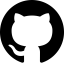
\includegraphics[width=0.05\linewidth]{github.png}
\end{textblock*}
\begin{textblock*}{350pt}(70pt, 205pt)
\href{https://github.com/tkoyama010}{@tkoyama010}
\end{textblock*}
\begin{textblock*}{350pt}(150pt, 25pt)
\begin{itemize}
\item Scientific simulation software engineer.
\note{
I am mechanical simulation software engineer in my careers.

私は科学シミュレーションのソフトウェアエンジニアとして働いています。

}
\item Stuff of Scipy Japan 2020.
\note{
And I was a staff of Scipy Japan 2020.

そして、Scipy Japan 2020のスタッフを務めました。

}
\item PyVista developer team member.
\note{
Also I am a member of PyVista developer team.

また、PyVista開発チームのメンバーでもあります。

}
\item Science, Python, Anime, and Manga.
\note{
I love Science, Python, Anime and Manga.

科学、Python、アニメ、マンガが大好きです。

}
\end{itemize}
\end{textblock*}
\begin{textblock*}{350pt}(200pt, 120pt)
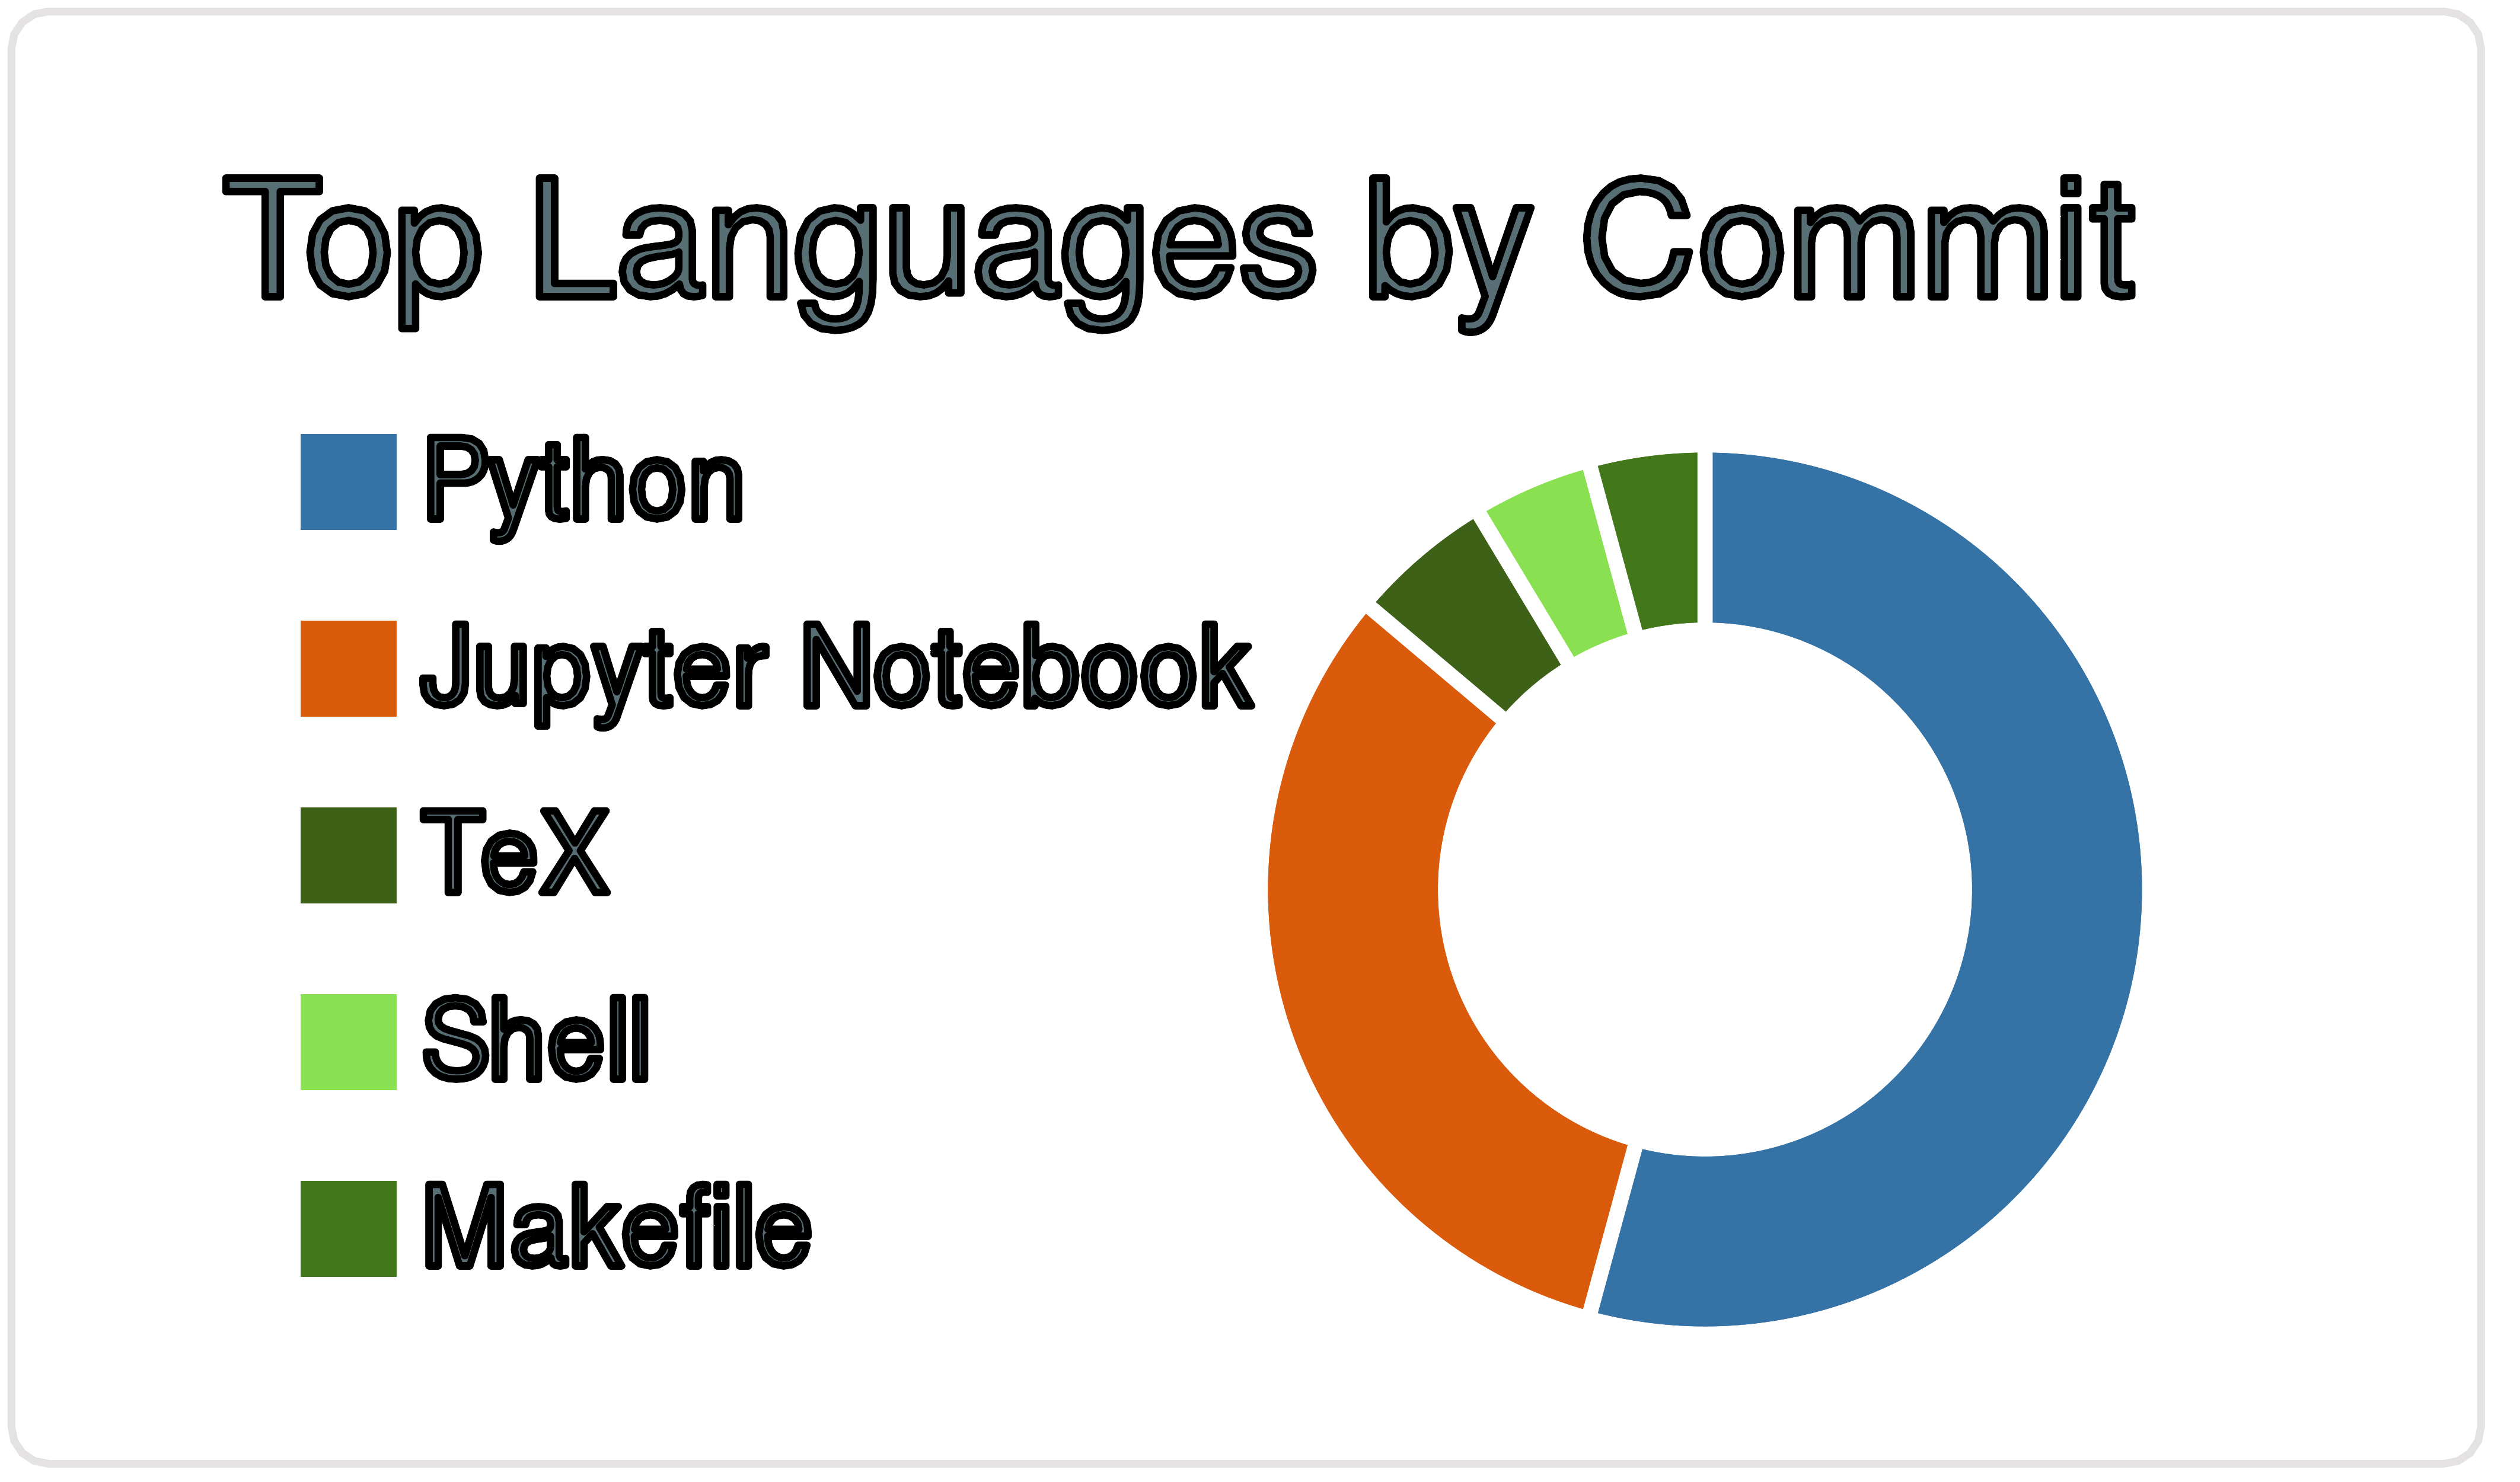
\includegraphics[width=0.50\linewidth]{2-most-commit-language.png}
\end{textblock*}
\note{
My Twitter and Github accounts are \href{https://twitter.com/tkoyama010}{@tkoyama010}.

私のTwitterとGithubのアカウントは\href{https://twitter.com/tkoyama010}{@tkoyama010}です。

}
\note{
Please follow me if you like this presentation.

このプレゼンテーションを気に入っていただけたら、ぜひフォローしてください。
}
\end{frame}

\begin{frame}[fragile]
\begin{textblock*}{800pt}(50pt, 10pt)
\begin{block}{What we want to do is using VTK like matplotlib in PyVista.}
\note{
Do you want to visualize 3D data in a Pythonic way like matplotlib?
If you want, this slides is for you.
This slides is the introduction of \href{https://pypi.org/project/pyvista/}{PyVista}. It is

matplotlibのようにPythonicな方法で3Dデータを視覚化したいと思ったことはありませんか?
このスライドはそんなあなたのためのものです。
このスライドでは、\href{https://pypi.org/project/pyvista/}{PyVista}と呼ばれるライブラリを紹介します。
このライブラリには3つの特徴があります。

}
\begin{itemize}
\item "VTK for humans"\: a high-level API to the Visualization Toolkit (VTK)
\note[item]{
"VTK for humans"\: a high-level API to the Visualization Toolkit (VTK)

1つ目は"人間のためのVTK"\: 可視化ツールキット(VTK)の高レベルAPIです。

}
\item 3D plotting made simple and built for large/complex data geometries
\note[item]{
3D plotting made simple and built for large/complex data geometries

2つ目は大規模/複雑なデータ形状に対応した、シンプルな3Dプロッティング機能です。

}
\item mesh data structures and filtering methods for spatial datasets
\note[item]{
mesh data structures and filtering methods for spatial datasets

3つ目はメッシュデータと空間データのフィルタリングメソッドです。

}
\end{itemize}
\end{block}
\end{textblock*}
\begin{textblock*}{800pt}(50pt, 100pt)
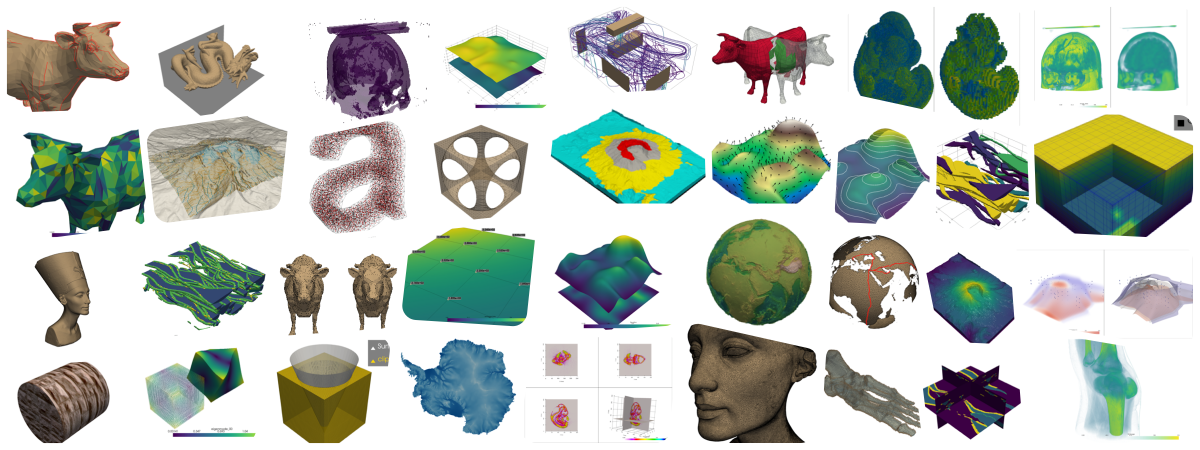
\includegraphics[width=0.50\linewidth]{pyvista_banner_small.png}
\end{textblock*}
\end{frame}

\begin{frame}[fragile]
\begin{textblock*}{350pt}(50pt, 10pt)
\begin{block}{Hello World!}
\lstinputlisting[caption=Hello World!, label=hello_world_code, firstline=1, lastline=100]{hello_world.py}
\end{block}
\end{textblock*}
\end{frame}
\note{
In Code Listing \ref{hello_world_code}, we demonstrate the "Hello World!" of \href{https://pypi.org/project/pyvista/}{PyVista}.
Basic step of \href{https://pypi.org/project/pyvista/}{PyVista} script is the following.
First, import \href{https://pypi.org/project/pyvista/}{PyVista}.
Then generate \href{https://dev.pyvista.org/getting-started/what-is-a-mesh.html}{mesh} and add it to
Plotter object using add mesh method.

コードリスト\ref{hello_world_code}では、\href{https://pypi.org/project/pyvista/}{PyVista}の "Hello World!" を行っています。
\href{https://pypi.org/project/pyvista/}{PyVista} スクリプトの基本ステップについて説明します。
まず、 \href{https://pypi.org/project/pyvista/}{PyVista} をインポートします。
次に \href{https://dev.pyvista.org/getting-started/what-is-a-mesh.html}{mesh} を生成して、それを
add meshメソッドを使用してPlotterオブジェクトに追加します。

}

\begin{frame}[fragile]
\begin{textblock*}{350pt}(50pt, 10pt)
\begin{block}{Hello World!}
\end{block}
\end{textblock*}
\begin{textblock*}{350pt}(50pt, 50pt)
\begin{block}{}
\begin{figure}
\includegraphics[width=1.0\linewidth]{hello_world.png}
\caption{Hello World!\label{HelloWorldFigure}}
\end{figure}
\note{
And finally, we can check the render view (Figure \ref{HelloWorldFigure}) of PyVista using show method.

最後に、showメソッドを使って、PyVistaのレンダリングビュー(図 \ref{HelloWorldFigure})を確認します。
}
\end{block}
\end{textblock*}
\end{frame}

\begin{frame}[fragile]
\begin{textblock*}{350pt}(50pt, 10pt)
\begin{block}{Create tube from line}
\lstinputlisting[caption=Create tube, label=CreateTube, firstline=15, lastline=15]{tube.py}
\begin{figure}
\includegraphics[width=1.0\linewidth]{tube.png}
\caption{Line and tube\label{LineTubeFigure}}
\end{figure}
\end{block}
\end{textblock*}
\end{frame}
\note{
We can also make customize mesh like tube from line points using Tube function.

Tube関数を使用して、線の点から管のようなメッシュをカスタマイズすることもできます。
}

\begin{frame}[fragile]
\begin{textblock*}{200pt}(50pt, 10pt)
\begin{block}{Create PolyData}
\lstinputlisting[caption=Create PolyData, label=CreatePolyDataCode, firstline=12, lastline=29]{create-poly.py}
\end{block}
\end{textblock*}
\begin{textblock*}{350pt}(180pt, 50pt)
\begin{figure}
\includegraphics[width=0.5\linewidth]{create-poly.png}
\caption{Create PolyData \label{CreatePolyData}}
\end{figure}
\end{textblock*}
\end{frame}
\note{
You can also create PolyData (Triangulated Surface) objects from the NumPy arrays of vertices and faces if you want to further customize the mesh.

メッシュをさらにカスタマイズする場合は、頂点と面のNumPy配列からPolyData (Triangulated Surface) オブジェクトを作成することもできます。

A PolyData object can be created quickly from numpy arrays.

PolyDataオブジェクトは、numpy配列からすばやく作成できます。

The vertex array contains the locations of the points in the mesh and the face array contains the number of points of each face and the indices of the vertices which comprise that face.

頂点配列にはメッシュ内のポイントの位置が含まれ、面配列には各面のポイント数と、その面を構成する頂点のインデックスが含まれます。

}

\begin{frame}[fragile]
\begin{textblock*}{350pt}(50pt, 10pt)
\begin{block}{Load and plot from a files}
\lstinputlisting[caption=Load meshs from the many supported file formats, label=ReadFileCode, firstline=5, lastline=8]{read_file.py}
\begin{figure}
\includegraphics[width=0.6\linewidth]{read_file.png}
\caption{Meshs from the many supported file formats\label{ReadFileFigure}}
\end{figure}
\end{block}
\end{textblock*}
\end{frame}
\note{
We can also load mesh from file.
Loading a \href{https://dev.pyvista.org/getting-started/what-is-a-mesh.html}{mesh} is trivial - if your data is in one of the many supported file formats,
simply use \href{https://dev.pyvista.org/utilities/utilities.html}{pyvista.read()}
to load your spatially referenced dataset into a \href{https://pypi.org/project/pyvista/}{PyVista} \href{https://dev.pyvista.org/getting-started/what-is-a-mesh.html}{mesh} object
(Code Listing \ref{ReadFileCode}, Figure \ref{ReadFileFigure}).

ファイルからメッシュをロードすることもできます。
\href{https://dev.pyvista.org/getting-started/what-is-a-mesh.html}{mesh} のロードは簡単です。
データがサポートされている多くのファイルフォーマットのいずれかである場合、
単に \href{https://dev.pyvista.org/utilities/utilities.html}{pyvista.read()} を使用して空間的に参照されたデータセットを
\href{https://pypi.org/project/pyvista/}{PyVista} \href{https://dev.pyvista.org/getting-started/what-is-a-mesh.html}{mesh} オブジェクトにロードします
(コードリスト\ref{ReadFileCode}、図\ref{ReadFileFigure})。
}

\begin{frame}[fragile]
\begin{textblock*}{350pt}(50pt, 10pt)
\begin{block}{Load and plot from a files}
\lstinputlisting[caption=Save meshs to the many supported file formats, label=SaveFileCode, firstline=26, lastline=29]{read_file.py}
\begin{figure}
\includegraphics[width=0.6\linewidth]{read_file.png}
\caption{Meshs from the many supported file formats\label{ReadFileFigure}}
\end{figure}
\end{block}
\end{textblock*}
\end{frame}
\note{
Also note that we can export any \href{https://pypi.org/project/pyvista/}{PyVista} mesh to any file format supported by \href{https://pypi.org/project/meshio/}{meshio}.

また、任意の \href{https://pypi.org/project/pyvista/}{PyVista} メッシュを \href{https://pypi.org/project/meshio/}{meshio} でサポートされている任意のファイルフォーマットにエクスポートできることにも注意してください。

To save a \href{https://pypi.org/project/pyvista/}{PyVista} mesh using meshio, use \href{https://dev.pyvista.org/utilities/utilities.html}{pyvista.save\_meshio()}(Code Listing \ref{SaveFileCode}):

meshioを使って \href{https://pypi.org/project/pyvista/}{PyVista} のメッシュを保存するには、 \href{https://dev.pyvista.org/utilities/utilities.html}{pyvista.save\_meshio()} を使います(コードリスト \ref{SaveFileCode} )。
}

\begin{frame}[fragile]
\begin{textblock*}{350pt}(50pt, 10pt)
\begin{block}{Thresholding Filter}
\lstinputlisting[caption=Create tube, label=ThresholdingFilterCode, firstline=36, lastline=36]{using-filters.py}
\begin{figure}
\includegraphics[width=1.0\linewidth]{using-filters1.png}
\caption{Thresholding\label{ThresholdingFilterFigure}}
\end{figure}
\end{block}
\end{textblock*}
\end{frame}
\note{
In this slide we use common filters like thresholding and clipping.
PyVista wrapped data objects have a suite of common filters ready for immediate use directly on the object.
These filters include the following (see Filters for a complete list).
To use these filters, call the method of your choice directly on your data object.
And now there is a thresholded version of the input dataset in the new threshed object.
To learn more about what keyword arguments are available to alter how filters are executed,
print the docstring for any filter attached to PyVista objects with either help or using shift+tab in an IPython environment.

このスライドではしきい値設定やクリッピングなどの一般的なフィルタを使用してみます。
PyVistaでラップされたデータオブジェクトには、オブジェクト上で直接すぐに使用できる一連の共通フィルタが用意されています。
これらのフィルタを使用するには、データ・オブジェクトで直接選択したメソッドを呼び出します。
これで、新しいしきい値オブジェクトに入力データセットのしきい値バージョンがあります。
フィルタの実行方法を変更するために使用できるキーワード引数の詳細については、ヘルプを使用するか、
IPython環境でshift+tabを使用して、PyVistaオブジェクトに適用されているフィルタのdocstringを出力してください。

}

\begin{frame}[fragile]
\begin{textblock*}{200pt}(20pt, 10pt)
\begin{block}{Using Common Filters}
\lstinputlisting[caption=Using Common Filters, label=using_common_filters, firstline=68, lastline=87]{using-filters.py}
\end{block}
\end{textblock*}
\begin{textblock*}{200pt}(250pt, 0pt)
\begin{figure}
\includegraphics[width=1.0\linewidth]{using-filters2.png}
\caption{Using Common Filters\label{UsingCommonFiltersFigure}}
\end{figure}
\end{textblock*}
\end{frame}
\note{
What about other filters?
Let’s collect a few filter results and compare them:
This is the figure of threshold, contour, slices and glyphs.

他のフィルターはどうですか?
いくつかのフィルタ結果を収集して比較します。
これはしきい値、コンター、スライス、グリフの図です。

}


\begin{frame}[fragile]
\begin{textblock*}{200pt}(20pt, 10pt)
\begin{block}{Filter Pipeline}
\lstinputlisting[caption=Filter Pipeline, label=using_common_filters, firstline=106, lastline=111]{using-filters.py}
\end{block}
\end{textblock*}
\begin{textblock*}{200pt}(250pt, 50pt)
\begin{figure}
\includegraphics[width=1.0\linewidth]{using-filters3.png}
\caption{Filter Pipeline\label{FilterPipelineFigure}}
\end{figure}
\end{textblock*}
\end{frame}

\note{
In PyVista, we can mimic the filtering pipeline through a chain; attaching each filter to the last filter.
In this example, several filters are chained together.
First, and empty threshold filter to clean out any NaN values.
Second, use an elevation filter to generate scalar values corresponding to height.
Then, use the clip filter to cut the dataset in half.
At the end, create three slices along each axial plane using the slice\_orthogonal filter.
And to view this filtered data, simply call the plot method (result.plot()) or create a rendering scene:

PyVistaでは、チェーンを介してフィルタリングパイプラインを模倣することができます。
各フィルタを最後のフィルタにアタッチします。
この例では、複数のフィルタが連結されています。
まず、すべてのNaN値を消去する空のしきい値フィルタです。
次に、高度フィルタを使用して、高さに対応するスカラー値を生成します。
さらに、クリップフィルタを使用してデータセットを半分にカットします。
最後に、slice\_orthogonalフィルタを使用して、各軸平面に沿って3つのスライスを作成します。
フィルタされたデータを表示するには、plotメソッド (result.plot () ) を呼び出すか、レンダリングシーンを作成します。
}

\begin{frame}[fragile]
\begin{textblock*}{350pt}(50pt, 10pt)
\begin{block}{Shrink mesh}
\lstinputlisting[caption=Shrink Mesh, label=ShrinkFilterCode, firstline=5, lastline=6]{shrunk_mesh.py}
\begin{figure}
\includegraphics[width=1.0\linewidth]{shrink.png}
\caption{Shrink filter\label{ShrinkFilterFigure}}
\end{figure}
\end{block}
\end{textblock*}
\end{frame}
\note{
There is also a filter useful for mesh viewing.
Code Listing \ref{ShrinkFilterCode} shrink the individual faces of a mesh using shrink method (Figure \ref{ShrinkFilterFigure}).

メッシュの確認に便利なフィルターもあります。
コードリスト \ref{ShrinkFilterCode} では、shrinkメソッドを使ってメッシュの各面を縮小しています(図 \ref{ShrinkFilterFigure})。
}

\begin{frame}[fragile]
\begin{textblock*}{350pt}(50pt, 10pt)
\begin{block}{Clip with Plane}
\lstinputlisting[caption=Clip with Plane, label=ClipWithPlaneCode, firstline=20, lastline=21]{clipping.py}
\begin{figure}
\includegraphics[width=1.0\linewidth]{clipping1.png}
\caption{Clip with Plane\label{ClipWithPlane}}
\end{figure}
\end{block}
\end{textblock*}
\end{frame}
\note{
We can also clip any dataset by a user defined plane using the pyvista.DataSetFilters.clip() filter

pyvistaを使用して、pyvista.DataSetFilters.clip() フィルタを使うことで、ユーザ定義平面によりデータセットをクリップすることもできます。
}

\begin{frame}[fragile]
\begin{textblock*}{350pt}(50pt, 10pt)
\begin{block}{Clip with Bounds}
\lstinputlisting[caption=Clip with Bounds, label=ClipWithBoundsCode, firstline=39, lastline=42]{clipping.py}
\begin{figure}
\includegraphics[width=1.0\linewidth]{clipping2.png}
\caption{Clip with Bounds\label{ClipWithBounds}}
\end{figure}
\end{block}
\end{textblock*}
\end{frame}
\note{
Clip any dataset by a set of XYZ bounds using the pyvista.DataSetFilters.clip\_box() filter.

pyvistaを使用して、XYZ境界のセットによってデータセットをクリップします。
DataSetFilters.clip\_box () フィルタです。

}

\begin{frame}[fragile]
\begin{textblock*}{350pt}(50pt, 10pt)
\begin{block}{Rotation about the x axis}
\note{
We can of course rotate the mesh about the axes.

もちろん、軸を中心にメッシュを回転させることもできます。

Let's rotate a mesh about its axes.

メッシュを軸周りに回転させてみましょう。

In this model, the x axis is from the left to right; the y axis is from bottom to top; and the z axis emerges from the image.

このモデルでは、x軸は左から右へ、y軸は下から上へ、z軸は画面から垂直になっています。

The camera location is the same in two images.

カメラの位置は2つの画像で同じです。

Rotate the mesh about the x axis every 60 degrees and we can plot it.

このメッシュをx軸を中心に60度ごとに回転させてプロットできます。

Of cource, we can plot also about other axis.

もちろん、他の軸についてもプロットできます。

}
\end{block}
\lstinputlisting[caption=X-Axis Rotation, firstline=66, lastline=69]{rotate.py}
\begin{figure}
\includegraphics[width=1.0\linewidth]{rotate_x.png}
\caption{X-Axis Rotation}
\end{figure}
\end{textblock*}
\end{frame}

\begin{frame}[fragile]
\begin{textblock*}{350pt}(50pt, 10pt)
\begin{block}{Rotation about the y axis}
\note{
Plot the mesh rotated about the y axis every 60 degrees.

メッシュを60度ごとにY軸を中心に回転させてプロットします。

Add the axes actor to the Plotter and set the axes origin to the point of rotation.

プロッターに軸アクターを追加し、軸の原点を回転点に設定しています。

}
\end{block}
\lstinputlisting[caption=Y-Axis Rotation, firstline=66, lastline=69]{rotate.py}
\begin{figure}
\includegraphics[width=1.0\linewidth]{rotate_y.png}
\caption{Y-Axis Rotation}
\end{figure}
\end{textblock*}
\end{frame}

\begin{frame}[fragile]
\begin{textblock*}{350pt}(50pt, 10pt)
\begin{block}{Rotation about the z axis}
\note{
Plot the mesh rotated about the z axis every 60 degrees.

メッシュを60度ごとにz軸を中心に回転させてプロットします。

Add the axes actor to the Plotter and set the axes origin to the point of rotation.

プロッターに軸アクターを追加し、軸の原点を回転点に設定しています。

}
\end{block}
\lstinputlisting[caption=Z-Axis Rotation, firstline=66, lastline=69]{rotate.py}
\begin{figure}
\includegraphics[width=1.0\linewidth]{rotate_z.png}
\caption{Z-Axis Rotation}
\end{figure}
\end{textblock*}
\end{frame}

\begin{frame}[fragile]
\begin{textblock*}{350pt}(50pt, 10pt)
\begin{block}{Rotation about a custom vector}
\note{
Plot the mesh rotated about a custom vector every 60 degrees.

メッシュを60度ごとのカスタムベクトルで回転させてプロットします。

Add the axes actor to the Plotter and set axes origin to the point of rotation.

プロッターに軸アクターを追加し、軸の原点を回転点に設定しています。

}
\end{block}
\lstinputlisting[caption=Custom Rotation, firstline=66, lastline=69]{rotate.py}
\begin{figure}
\includegraphics[width=1.0\linewidth]{rotate_custom.png}
\caption{Custom Rotation}
\end{figure}
\end{textblock*}
\end{frame}

\begin{frame}[fragile]
\begin{textblock*}{350pt}(50pt, 10pt)
\begin{block}{General filters to any data type}
\lstinputlisting[caption=Extrude Rotate, label=ExtrudeRotateCode, firstline=7, lastline=9]{extrude_rotate.py}
\begin{figure}
\includegraphics[width=1.0\linewidth]{extrude_rotate.png}
\caption{Extrude Rotation\label{ExtrudeRotateFigure}}
\end{figure}
\note{
Code Listing \ref{ExtrudeRotateCode}  creating "skirt" from line
using extrude rotate method (Figure \ref{ExtrudeRotateFigure}).

コードリスト \ref{ExtrudeRotateCode} では、押出し回転メソッドを使って直線から "skirt" を
作成しています (図\ref{ExtrudeRotateFigure}) 。
}
\end{block}
\end{textblock*}
\end{frame}

\begin{frame}[fragile]
\begin{textblock*}{350pt}(50pt, 10pt)
\begin{block}{Extracting and Contouring}
\lstinputlisting[caption=Extracted by scalar, label=WarpScalarCode, firstline=9, lastline=9]{contour.py}
\begin{figure}
\includegraphics[width=0.5\linewidth]{contour.png}
\caption{Contouring\label{WarpScalarFigure}}
\end{figure}
\note{
Attributes are data values that live on either the nodes or cells of a mesh.

Attributeとは、メッシュのノードまたはセル上に存在するデータ値のことです。

In \href{https://pypi.org/project/pyvista/}{PyVista}, we work with both point data and cell data and allow easy access to data dictionaries to hold arrays for attributes that live either on all nodes or on all cells of a mesh.

\href{https://pypi.org/project/pyvista/}{PyVista} では、ポイントデータとセルデータの両方を扱い、メッシュのすべてのノードまたはすべてのセルに存在する属性の配列を保持するデータ辞書に簡単にアクセスできるようにしています。

Meshes can have a scalar field extracted using \href{https://dev.pyvista.org/core/filters.html}{warp\_by\_scalar()} method (Code List \ref{WarpScalarCode}, Figure \ref{WarpScalarFigure}).

\href{https://dev.pyvista.org/core/filters.html}{warp\_by\_scalar()} メソッドでメッシュからスカラーフィールドを抽出することができます(コードリスト \ref{WarpScalarCode} 、図 \ref{WarpScalarFigure} )。

}
\end{block}
\end{textblock*}
\end{frame}

\begin{frame}[fragile]
\begin{textblock*}{350pt}(50pt, 10pt)
\begin{block}{Plot data over circular arc}
\lstinputlisting[caption=Plotting over circular arc, label=PlotOverCircularArcCode, firstline=10, lastline=18]{kitchen.py}
\end{block}
\end{textblock*}
\begin{textblock*}{300pt}(0pt, 110pt)
\begin{block}{}
\note{
It can be plotting the values of a dataset over a circular arc through that dataset using
\href{https://dev.pyvista.org/core/filters.html}{plot\_over\_circular\_arc\_normal}
(Code list \ref{PlotOverCircularArcCode}, Figure \ref{CircularArcToPlotFigure} and \ref{PlotOverCircularArcFigure}).

\href{https://dev.pyvista.org/core/filters.html}{plot\_over\_circular\_arc\_normal}
を使用して、データセットを通る円弧上のデータセットの値をプロットすることができます
(コードリスト\ref{PlotOverCircularArcCode}、図\ref{CircularArcToPlotFigure}および\ref{PlotOverCircularArcFigure})。

}
\begin{figure}
\includegraphics[width=0.5\linewidth]{kitchen.png}
\caption{Circular arc to plot \label{CircularArcToPlotFigure}}
\end{figure}
\end{block}
\end{textblock*}
\begin{textblock*}{350pt}(150pt, 130pt)
\begin{figure}
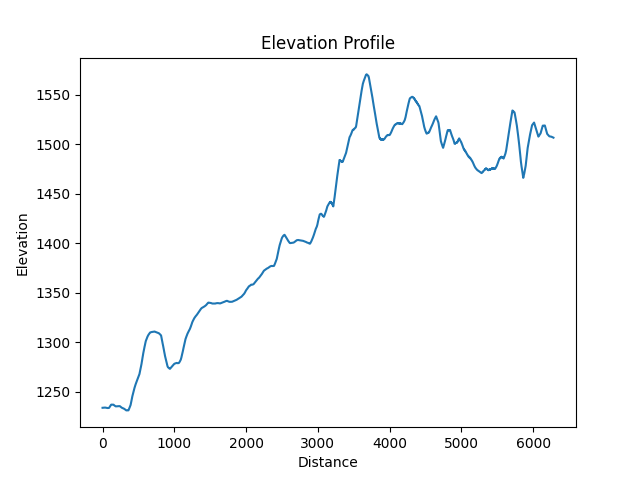
\includegraphics[width=0.3\linewidth]{elevation.png}
\caption{Plot over line \label{PlotOverCircularArcFigure}}
\end{figure}
\end{textblock*}
\end{frame}

\begin{frame}[fragile]
\begin{textblock*}{350pt}(50pt, 10pt)
\begin{block}{Extracting and Contouring}
\lstinputlisting[caption=Extracted by vector, label=WarpVectorCode, firstline=44, lastline=44]{contour.py}
\begin{figure}
\includegraphics[width=1.0\linewidth]{warped_vector.png}
\caption{Warped sphere by vector\label{WarpVectorFigure}}
\end{figure}
\end{block}
\end{textblock*}
\end{frame}
\note{
Also can have a vector filed extracted using \href{https://dev.pyvista.org/core/filters.html}{warp\_by\_vector()} method (Code List \ref{WarpVectorCode}, Figure \ref{WarpVectorFigure}).

また、 \href{https://dev.pyvista.org/core/filters.html}{warp\_by\_vector()} メソッドで抽出されたベクターファイルを持つことができます(コードリスト \ref{WarpVectorCode} 、図 \ref{WarpVectorFigure} )。

\href{https://dev.pyvista.org/plotting/plotting.html}{add\_mesh()} method can use a Matplotlib, Colorcet, cmocean, or custom colormap when plotting scalar values(Figure \ref{WarpVectorFigure}).

\href{https://dev.pyvista.org/plotting/plotting.html}{add\_mesh () }メソッドは、スカラー値をプロットするときにMatplotlib、Colorcet、cmocean、またはカスタムカラーマップを使用できます (図\ref{WarpVectorFigure}) 。

}

\begin{frame}[fragile]
\begin{textblock*}{350pt}(50pt, 10pt)
\begin{block}{Silhouette Highlight}
\lstinputlisting[caption=Silhouette Highlight, label=SilhouetteHighlight, firstline=22, lastline=28]{silhouette.py}
\begin{figure}
\includegraphics[width=1.0\linewidth]{silhouette1.png}
\caption{Silhouette Highlight\label{WarpVectorFigure}}
\end{figure}
\end{block}
\end{textblock*}
\end{frame}
\note{
We can extract a subset of the edges of a polygonal mesh to generate an outline silhouette of a mesh using add\_mesh method.
We can set it using the silhouette argument.

ポリゴンメッシュのエッジのサブセットを抽出し、add\_meshメソッドを使用してメッシュのアウトラインシルエットを生成できます。
シルエット引数で設定することができます。
}

\begin{frame}[fragile]
\begin{textblock*}{350pt}(50pt, 10pt)
\begin{block}{Camera class}
\begin{figure}
\includegraphics[width=0.75\linewidth]{frustum_of_camera.png}
\caption{Frustum of camera \label{CameraFrustumFigure}}
\end{figure}
\note{
Add a background image with pyvista.Plotter.add\_background\_image().
\href{https://dev.pyvista.org/core/camera.html}{Camera} class is a virtual camera for 3D rendering.

\href{https://dev.pyvista.org/core/camera.html}{Camera}クラスは、3Dレンダリング用の仮想カメラです。

It provides methods to position and orient the view point and focal point.

視点や焦点の位置や方向を決めるメソッドを提供します。

Convenience methods for moving about the focal point also are provided.

また、焦点を移動するための便利なメソッドも提供されています。

More complex methods allow the manipulation of the computer graphics model including view up vector, clipping planes, and camera perspective (Figure \ref{CameraFrustumFigure}).

より複雑なメソッドでは、ビューアップベクター、クリッピングプレーン、カメラパースペクティブなど、コンピュータグラフィックスモデルを操作することができます(図 \ref{CameraFrustumFigure})。

}
\lstinputlisting[caption=Add Camera to Plotter, label=camera_view, firstline=7, lastline=13]{camera_view.py}
\end{block}
\end{textblock*}
\end{frame}

\begin{frame}[fragile]
\begin{textblock*}{350pt}(50pt, 10pt)
\begin{block}{Camera class}
\lstinputlisting[caption=Create camera frustum, label=CameraFrustumCode, firstline=8, lastline=13]{frustum_of_camera.py}
\begin{figure}
\includegraphics[width=0.75\linewidth]{camera_view.png}
\caption{Camera view}
\end{figure}
\note{
Code Listing \ref{CameraFrustumCode} create a camera and frustum.

コードリスト\ref{CameraFrustumCode}ではカメラと視錐台を作成しています。

Then create a scene of inside frustum adding \href{https://dev.pyvista.org/core/camera.html}{Camera} object to \href{https://dev.pyvista.org/plotting/plotting.html}{Plotter} object
(Code list \ref{CameraFrustumCode} ,Figure \ref{CameraFrustumFigure}).

次に、視錐台内部のシーンを作成して、\href{https://dev.pyvista.org/plotting/plotting.html}{Plotter}オブジェクトに\href{https://dev.pyvista.org/core/camera.html}{Camera}オブジェクトを追加します
(コードリスト\ref{CameraFrustumCode}、図\ref{CameraFrustumFigure})。

}
\end{block}
\end{textblock*}
\end{frame}

\begin{frame}[fragile]
\begin{textblock*}{150pt}(50pt, 10pt)
\begin{block}{Controlling Camera Rotation}
\lstinputlisting[caption=Controlling Camera Rotation, label=CameraRotationCode, firstline=29, lastline=29]{camera_view.py}
\lstinputlisting[firstline=34, lastline=34]{camera_view.py}
\lstinputlisting[firstline=39, lastline=39]{camera_view.py}
\end{block}
\end{textblock*}
\begin{textblock*}{350pt}(150pt, 50pt)
\begin{figure}
\includegraphics[width=0.5\linewidth]{camera_rotation.png}
\caption{Controlling Camera Rotation \label{CameraRotationFigure}}
\end{figure}
\note{
In addition to directly controlling the camera position by setting it via the pyvista
\href{https://dev.pyvista.org/core/camera.html}{Camera.position}
property

さらに、pyvistaの\href{https://dev.pyvista.org/core/camera.html}{Camera.position}
プロパティを使用してカメラ位置を設定することにより、カメラ位置を直接制御することもできます。

You can also directly control the
\href{https://dev.pyvista.org/core/camera.html}{pyvista.Camera.roll},
\href{https://dev.pyvista.org/core/camera.html}{pyvista.Camera.elevation}, and
\href{https://dev.pyvista.org/core/camera.html}{pyvista.Camera.azimuth}
of the camera.
(Code list \ref{CameraRotationCode} ,Figure \ref{CameraRotationFigure}).

カメラの
\href{https://dev.pyvista.org/core/camera.html}{pyvista.Camera.roll},
\href{https://dev.pyvista.org/core/camera.html}{pyvista.Camera.elevation},
および\href{https://dev.pyvista.org/core/camera.html}{pyvista.Camera.azimuth}
を直接制御することもできます。
(コードリスト\ref{CameraRotationCode}、図\ref{CameraRotationFigure})

}
\end{textblock*}
\end{frame}

\begin{frame}[fragile]
\begin{textblock*}{350pt}(50pt, 10pt)
\begin{block}{Light Types}
\lstinputlisting[caption=Headlight, label=Headlight, firstline=32, lastline=36]{light_types.py}
\begin{figure}
\includegraphics[width=1.0\linewidth]{light_types1.png}
\caption{Headlight\label{Headlight}}
\end{figure}
\end{block}
\end{textblock*}
\end{frame}
\note{
We can also set the condition of the light.
Lights come in three types:

光の状態を設定することもできます。
光源には3つのタイプがあります。

First type is headlight.
The axis of which always coincides with the view of the camera,
For headlights the position and focal\_point properties are meaningless. 
No matter where you move the camera, the light always emanates from the view point:

1つ目はヘッドライトです。
軸は常にカメラのビューと一致します。
ヘッドライトの場合、positionプロパティとfocal\_pointプロパティは意味がありません。
カメラをどこに移動しても、ライトは常に視点から放射されます。
}

\begin{frame}[fragile]
\begin{textblock*}{350pt}(50pt, 10pt)
\begin{block}{Light Types}
\lstinputlisting[caption=Cameralight, label=Cameralight, firstline=54, lastline=56]{light_types.py}
\begin{figure}
\includegraphics[width=1.0\linewidth]{light_types2.png}
\caption{Cameralight\label{Cameralight}}
\end{figure}
\end{block}
\end{textblock*}
\end{frame}
\note{
Second is camera light.
Camera lights define their position and focal\_point properties in a coordinate system that is local to the camera.
The coordinates in the scene’s coordinate system can be accessed through the world\_position and world\_focal\_point read-only properties, respectively.
For specifics of the local coordinate system used for the coordinates please see the documentation of pyvista.Light.set\_camera\_light().

2つ目はカメラライトです。カメラライトは、カメラに対してローカルな座標系で位置とfocal\_pointプロパティを定義します。
シーンの座標系の座標には、それぞれworld\_positionおよびworld\_focal\_point読み取り専用プロパティからアクセスできます。
座標に使用されるローカル座標系の詳細については、pyvistaLight.set\_camera\_light()のドキュメントを参照してください。
}

\begin{frame}[fragile]
\begin{textblock*}{350pt}(50pt, 10pt)
\begin{block}{Light Types}
\lstinputlisting[caption=Scenelight, label=Scenelight, firstline=69, lastline=71]{light_types.py}
\begin{figure}
\includegraphics[width=1.0\linewidth]{light_types3.png}
\caption{Scenelight\label{Scenelight}}
\end{figure}
\end{block}
\end{textblock*}
\end{frame}
\note{
Third is scene light.
Scene lights are attached to the scene, their position and focal point are
interpreted as global coordinates:

3つ目はシーンライトです。
シーンライトはシーンにアタッチされ、その位置と焦点はグローバル座標として解釈されます。

}

\begin{frame}[fragile]
\begin{textblock*}{350pt}(50pt, 10pt)
\begin{block}{Eye Dome Lighting}
\end{block}
\end{textblock*}
\end{frame}
\note{
Eye-Dome Lighting (EDL) is a non-photorealistic, image-based shading technique designed to improve depth perception in scientific visualization images.
Eye-Dome Lighting can dramatically improve depth perception when plotting incredibly sophisticated meshes like the creative commons Queen Nefertiti statue:
Here we will compare a EDL shading side by side with normal shading
}

\begin{frame}[fragile]
\begin{textblock*}{350pt}(50pt, 10pt)
\begin{block}{Point Cloud}
\end{block}
\end{textblock*}
\end{frame}
\note{
When plotting a simple point cloud, it can be difficult to perceive depth. Take this Lidar point cloud for example:
And now plot this point cloud as-is:
We can improve the depth mapping by enabling eye dome lighting on the renderer with pyvista.Renderer.enable\_eye\_dome\_lighting().
The eye dome lighting mode can also handle plotting scalar arrays:
}

\begin{frame}[fragile]
\begin{textblock*}{350pt}(50pt, 10pt)
\begin{block}{Geodesic Paths}
\end{block}
\end{textblock*}
\end{frame}
\note{
Calculates the geodesic path between two vertices using Dijkstra’s algorithm
Get the geodesic path as a new pyvista.PolyData object:
Render the path along the land surface
How long is that path?
}

\begin{frame}[fragile]
\begin{textblock*}{350pt}(50pt, 10pt)
\begin{block}{Applying Textures}
\end{block}
\end{textblock*}
\end{frame}
\note{
Plot a mesh with an image projected onto it as a texture.
Texture mapping is easily implemented using PyVista.
Many of the geometric objects come preloaded with texture coordinates, so quickly creating a surface and displaying an image is simply:
But what if your dataset doesn’t have texture coordinates? Then you can harness the pyvista.
DataSetFilters.texture\_map\_to\_plane() filter to properly map an image to a dataset’s surface.
For example, let’s map that same image of bricks to a curvey surface:
Display scalar data along with a texture by ensuring the interpolate\_before\_map setting is False and specifying both the texture and scalars arguments.
Note that this process can be completed with any image texture!
}

\begin{frame}[fragile]
\begin{textblock*}{350pt}(50pt, 10pt)
\begin{block}{Textures from Files}
\end{block}
\end{textblock*}
\end{frame}
\note{
What about loading your own texture from an image?
This is often most easily done using the pyvista.read\_texture() function - simply pass an image file’s path, and this function with handle making a vtkTexture for you to use.
}

\begin{frame}[fragile]
\begin{textblock*}{350pt}(50pt, 10pt)
\begin{block}{NumPy Arrays as Textures}
\end{block}
\end{textblock*}
\end{frame}
\note{
Want to use a programmatically built image?
pyvista.UniformGrid objects can be converted to textures using pyvista.image\_to\_texture() and 3D NumPy (X by Y by RGB) arrays can be converted to textures using pyvista.numpy\_to\_texture().
}

\begin{frame}[fragile]
\begin{textblock*}{350pt}(50pt, 10pt)
\begin{block}{Textures with Transparency}
\end{block}
\end{textblock*}
\end{frame}
\note{
Textures can also specify per-pixel opacity values.
The image must contain a 4th channel specifying the opacity value from 0 [transparent] to 255 [fully visible].
To enable this feature just pass the opacity array as the 4th channel of the image as a 3 dimensional matrix with shape [nrows, ncols, 4] pyvista.numpy\_to\_texture().
Here we can download an image that has an alpha channel:
}

\begin{frame}[fragile]
\begin{textblock*}{350pt}(50pt, 10pt)
\begin{block}{Repeating Textures}
\end{block}
\end{textblock*}
\end{frame}
\note{
What if you have a single texture that you’d like to repeat across a mesh?
Simply define the texture coordinates for all nodes explicitly.
Here we create the texture coordinates to fill up the grid with several mappings of a single texture.
In order to do this we must define texture coordinates outside of the typical (0, 1) range:
By defining texture coordinates that range (0, 4) on each axis, we will produce 4 repetitions of the same texture on this mesh.
Then we must associate those texture coordinates with the mesh through the pyvista.DataSet.active\_t\_coords property.
Now display all the puppies!
}

\begin{frame}[fragile]
\begin{textblock*}{350pt}(50pt, 10pt)
\begin{block}{Spherical Texture Coordinates}
\end{block}
\end{textblock*}
\end{frame}
\note{
We have a built in convienance method for mapping textures to spherical coordinate systems much like the planar mapping demoed above.
The helper method above does not always produce the desired texture coordinates, so sometimes it must be done manually. Here is a great, user contributed example from this support issue
Manually create the texture coordinates for a globe map. First, we create the mesh that will be used as the globe. Note the start\_theta for a slight overlappig
}

\begin{frame}[fragile]
\begin{textblock*}{350pt}(50pt, 10pt)
\begin{block}{Physically Based Rendering}
\end{block}
\end{textblock*}
\end{frame}
\note{

VTK 9 introduced Physically Based Rendering (PBR) and we have exposed that functionality in PyVista. Read the blog about PBR for more details.

PBR is only supported for pyvista.PolyData and can be triggered via the pbr keyword argument of add\_mesh. Also use the metallic and roughness arguments for further control.

Let’s show off this functionality by rendering a high quality mesh of a statue as though it were metallic.

Let’s render the mesh with a base color of “linen” to give it a metal looking finish.

Show the variation of the metallic and roughness parameters.

Plot with metallic increasing from left to right and roughness increasing from bottom to top.

Combine custom lighting and physically based rendering.

}

\begin{frame}[fragile]
\begin{textblock*}{350pt}(50pt, 10pt)
\begin{block}{Working with a glTF Files}
\end{block}
\end{textblock*}
\end{frame}
\note{
Import a glTF directly into a PyVista plotting scene. For more details regarding the glTF format, see: https://www.khronos.org/gltf/
Note this feature is only available for vtk>=9.
First, download the examples. Note that here we’re using a high dynamic range texture since glTF files generally contain physically based rendering and VTK v9 supports high dynamic range textures.
Setup the plotter and enable environment textures. This works well for physically based rendering enabled meshes like the damaged helmet example.
You can also directly read in gltf files and extract the underlying mesh.
}

\begin{frame}[fragile]
\begin{block}{Widgets}
\end{block}
\end{frame}
\note{
PyVista has several widgets that can be added to the rendering scene to control filters like clipping, slicing, and thresholding - specifically there are widgets to control the positions of boxes, planes, and lines or slider bars which can all be highly customized through the use of custom callback functions.
Here we’ll take a look at the various widgets, some helper methods that leverage those widgets to do common tasks, and demonstrate how to leverage the widgets for user defined tasks and processing routines.
}

\begin{frame}[fragile]
\begin{block}{Widgets}
\movie[width=5cm,height=5cm]{}{box-clip.gif}
\end{block}
\end{frame}
\note{
The box widget can be enabled and disabled by the pyvista.WidgetHelper.add\_box\_widget() and pyvista.WidgetHelper.clear\_box\_widgets() methods respectively.
When enabling the box widget, you must provide a custom callback function otherwise the box would appear and do nothing - the callback functions are what allow us to leverage the widget to perform a task like clipping/cropping.

Considering that using a box to clip/crop a mesh is one of the most common use cases, we have included a helper method that will allow you to add a mesh to a scene with a box widget that controls its extent, the pyvista.WidgetHelper.add\_mesh\_clip\_box() method.
}

\begin{frame}[fragile]
\begin{block}{Plane Widget}
\end{block}
\end{frame}
\note{
The plane widget can be enabled and disabled by the pyvista.WidgetHelper.add\_plane\_widget() and pyvista.WidgetHelper.clear\_plane\_widgets() methods respectively.
As with all widgets, you must provide a custom callback method to utilize that plane.
Considering that planes are most commonly used for clipping and slicing meshes, we have included two helper methods for doing those tasks!
Let’s use a plane to clip a mesh:
After interacting with the scene, the clipped mesh is available as:
And here is a screen capture of a user interacting with this
Or you could slice a mesh using the plane widget:
After interacting with the scene, the slice is available as:
And here is a screen capture of a user interacting with this
}

\begin{frame}[fragile]
\begin{block}{Slider Widget}
\end{block}
\end{frame}
\note{
The slider widget can be enabled and disabled by the pyvista.WidgetHelper.add\_slider\_widget() and pyvista.WidgetHelper.clear\_slider\_widgets() methods respectively.
This is one of the most versatile widgets as it can control a value that can be used for just about anything.
One helper method we’ve added is the pyvista.WidgetHelper.add\_mesh\_threshold() method which leverages the slider widget to control a thresholding value.
After interacting with the scene, the threshold mesh is available as:
Or you could leverage a custom callback function that takes a single value from the slider as its argument to do something like control the resolution of a mesh. Again note the use of the name argument in add\_mesh:
And here is a screen capture of a user interacting with this
}

\begin{frame}[fragile]
\begin{block}{Sphere Widget}
\end{block}
\end{frame}
\note{
The sphere widget can be enabled and disabled by the pyvista.WidgetHelper.add\_sphere\_widget() and pyvista.WidgetHelper.clear\_sphere\_widgets() methods respectively. This is a very versatile widget as it can control vertex location that can be used to control or update the location of just about anything.
We don’t have any convenient helper methods that utilize this widget out of the box, but we have added a lot of ways to use this widget so that you can easily add several widgets to a scene.
Let’s look at a few use cases that all update a surface mesh.
}

\begin{frame}[fragile]
\begin{block}{Interpolate Before Mapping}
\end{block}
\end{frame}
\note{
The add\_mesh function has an interpolate\_before\_map argument - this affects the way scalar data is visualized with colors. The effect can of this can vary depending on the dataset’s topology and the chosen colormap.
This example serves to demo the difference and why we’ve chosen to enable this by default.
For more details, please see this blog post

Meshes are colored by the data on their nodes or cells - when coloring a mesh by data on its nodes, the values must be interpolated across the faces of cells. The process by which those scalars are interpolated is critical. If the interpolate\_before\_map is left off, the color mapping occurs at polygon points and colors are interpolated, which is generally less accurate whereas if the interpolate\_before\_map is on, then the scalars will be interpolated across the topology of the dataset which is more accurate.

To summarize, when interpolate\_before\_map is off, the colors are interpolated after rendering and when interpolate\_before\_map is on, the scalars are interpolated across the mesh and those values are mapped to colors.

So lets take a look at the difference:
Shown in the figure above, when not interpolating the scalars before mapping, the colors (RGB values, not scalars) are interpolated between the vertices by the underlying graphics library (OpenGL), and the colors shown are not accurate.

The same interpolation effect occurs for wireframe visualization too:
The cylinder mesh above is a great example dataset for this as it has a wide spread between the vertices (points are only at the top and bottom of the cylinder) which means high surface are of the mesh has to be interpolated.

However, most meshes don’t have such a wide spread and the effects of color interpolating are harder to notice. Let’s take a look at a wavelet example and try to figure out how the interpolate\_before\_map option affects its rendering.

This time is pretty difficult to notice the differences - they are there, subtle, but present. The differences become more apparent when we decrease the number of colors in colormap. Let’s take a look at the differences when using eight discrete colors via the n\_colors argument:

Left, interpolate\_before\_map OFF. Right, interpolate\_before\_map ON.

Now that is much more compelling! On the right, the contours of the scalar field are visible, but on the left, the contours are obscured due to the color interpolation by OpenGL. In both cases, the colors at the vertices are the same, the difference is how color is assigned between the vertices.

In our opinion, color interpolation is not a preferred default for scientific visualization and is why we have chosen to set the interpolate\_before\_map flag to True.
}

\begin{frame}[fragile]
\begin{textblock*}{350pt}(50pt, 10pt)
\begin{block}{Acknowlegment}
I would like to thank \href{https://github.com/orgs/pyvista/teams/developers}{PyVista developer team} for developing useful library.
\end{block}
\begin{block}{References}
C. Bane Sullivan and Alexander Kaszynski, (2019). PyVista: 3D plotting and mesh analysis through a streamlined interface for the Visualization Toolkit (VTK). Journal of Open Source Software, 4(37), 1450, \url{https://doi.org/10.21105/joss.01450}
\end{block}
\begin{block}{Contact Information}
If you want to know and discuss pyvista more, join \href{http://github.com/pyvista/pyvista/discussions}{GitHub Discussion}.
\end{block}
\note{
I would like to thank PyVista developer team for developing useful library.

役に立つライブラリを開発してくれたPyVista開発チームに感謝します。

If you want to know and discuss pyvista more, join \href{http://github.com/pyvista/pyvista/discussions}{GitHub Discussion}.

pyvistaについてもっと知りたいなら、\href{http://github.com/pyvista/pyvista/discussions}{GitHub Discussion}に参加してください。

}
\doclicenseThis
\end{textblock*}
\end{frame}

\end{document}

